% Contributions are much appreciated, in order to contribute to this project, head over to this repository:
% https://github.com/bshramin/uofa-eng-assignment

\documentclass[11pt,letterpaper]{article}
\textwidth 6.5in
\textheight 9.in
\oddsidemargin 0in
\headheight 0in
\usepackage{graphicx}
\usepackage{fancybox}
\usepackage[utf8]{inputenc}
\usepackage{epsfig,graphicx}
\usepackage{multicol,pst-plot}
\usepackage{pstricks}
\usepackage{amsmath}
\usepackage{amsfonts}
\usepackage{amssymb}
\usepackage{eucal}
\usepackage[left=2cm,right=2cm,top=2cm,bottom=2cm]{geometry}
\usepackage{esvect}
\pagestyle{empty}
\DeclareMathOperator{\tr}{Tr}
\newcommand*{\op}[1]{\check{\mathbf#1}}
\newcommand{\bra}[1]{\langle #1 |}
\newcommand{\ket}[1]{| #1 \rangle}
\newcommand{\braket}[2]{\langle #1 | #2 \rangle}
\newcommand{\mean}[1]{\langle #1 \rangle}
\newcommand{\opvec}[1]{\check{\vec #1}}
\renewcommand{\sp}[1]{$${\begin{split}#1\end{split}}$$}

\usepackage{lipsum}

\usepackage{listings}
\usepackage{color}
\usepackage{wrapfig}
\usepackage[shortlabels]{enumitem}

\definecolor{codegreen}{rgb}{0,0.6,0}
\definecolor{codegray}{rgb}{0.5,0.5,0.5}
\definecolor{codepurple}{rgb}{0.58,0,0.82}
\definecolor{backcolour}{rgb}{0.95,0.95,0.92}

\lstdefinestyle{mystyle}{
	backgroundcolor=\color{backcolour},   
	commentstyle=\color{codegreen},
	keywordstyle=\color{magenta},
	numberstyle=\tiny\color{codegray},
	stringstyle=\color{codepurple},
	basicstyle=\footnotesize,
	breakatwhitespace=false,         
	breaklines=true,                 
	captionpos=b,                    
	keepspaces=true,                 
	numbers=left,                    
	numbersep=5pt,                  
	showspaces=false,                
	showstringspaces=false,
	showtabs=false,                  
	tabsize=2
}

\lstset{style=mystyle}

\begin{document}
\pagestyle{plain}

\begin{flushleft}
Estudiante: Fabio Quimbay\\
Email: fabio.quimbay883@comunidadunir.net\\
Profesor: Miguel Ángel Cabeza\\
Fecha: Noviembre 9 de 2022\\
\end{flushleft}

\begin{flushright}\vspace{-20mm}

\includegraphics[height=2cm]{logo.png}
\end{flushright}
 
\begin{center}\vspace{0cm}
\textbf{\large PER5786 2022-2023  Física 1 (GFI) - PER5786 2022-2023}\\
 Tema 2 - Cinemática
\end{center}

 
\rule{\linewidth}{0.1mm}
%%%%%%%%%%%%%%%%%%%%%%%%%%%%%%%%%%%%%%%%%%%%%%%%%%%%%%%%%%%%%%%%%%%%%%%%

\bigskip
\bigskip

%%%%%%%%%%%%%%%%%%%%
\textbf{Ejercicio 7 propuesto}\\

Calcula la aceleración centrípeta de la tierra orbitando alrededor del sol, y la aceleración centrípeta del sistema solar orbitando alrededor del centro de la Vía Láctea. Compara sus valores con la aceleración gravitatoria, $g=9.8 m/s^2$, en la superficie de la tierra.\\

\begin{figure}[h]
\centering
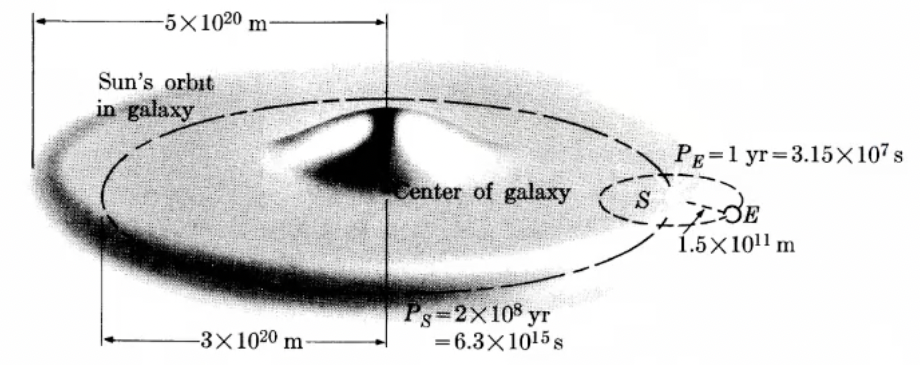
\includegraphics[width=0.5\textwidth]{ejemplo_7.png}
\end{figure}

Datos: 
\begin{itemize}
  \item Radio de giro del sol con respecto al centro de la Vía Láctea $Rs=5 \times 10^{20}$ m.
  \item Período de giro del sol con respecto al centro de la Vía Láctea $Ps=6.3 \times 10^{15}$ s.
  \item Radio de giro de la tierra con respecto al sol $Rt=1.5 \times 10^{11}$ m.
  \item Período de giro de la tierra con respecto al sol $Pt=3.15 \times 10^{7}$ s.
\end{itemize}

\textbf{Formulas base:}\\

Se tomarán las siguientes formulas base:

\begin{align}
\boxed{ a_{c} = \frac{v^2}{R} = \frac{{WR}^2}{R} = {\omega}^2 \cdot R}\\
\boxed{ T = \frac{2 \cdot \pi}{\omega} \Rightarrow \omega = \frac{2 \cdot \pi}{T}}
\end{align}

\textbf{Solución:}\\

Estos parámetros corresponden a los valores usados en el ejercicio propuesto, a saber:

\begin{align*}
R_{s} &= 5 \times {10}^20\,m \quad P_{s} = 6.3 \times {10}^15\,m\\
R_{t} &= 1.5 \times {10}^11\,m \quad P_{t} = 3.15 \times {10}^7\,m
\end{align*}

Primero se calcula la aceleración centrípeta de la tierra con relación al sol, a saber:

\begin{align*}
R_{s} &= 5 \times {10}^20\,m \quad P_{s} = 6.3 \times {10}^15\,m\\
R_{t} &= 1.5 \times {10}^11\,m \quad P_{t} = 3.15 \times {10}^7\,m
\end{align*}

\begin{align*}
a_{C_{T}} &= \frac{V_{ORB}^2}{R_{T}} = \frac{\omega^2 \cdot R_{T}^2}{R_{T}} = \frac{4 \cdot \pi^2}{T_{T}^2}\\
a_{C_{T}} &= \frac{4 \cdot \pi^2 \cdot 1.5 \times 10^{11}}{(3.15 \times 10^{7})^2} = 0.005968 = 5.968 \times 10^{-3}\,m/s\\
\,\\
a_{C_{S}} &= \frac{4 \cdot \pi^2 \cdot 5 \times 10^{20}}{(6.3 \times 10^{15})^2} = 4.97335 \times 10^{-10}\,m/s\\
\,\\
\frac{g}{a_{C_{T}}} &= \frac{9.8\,m/s^2}{5.968 \times 10^{-3}\,m/s^2} = 1642.09\\
\frac{g}{a_{C_{S}}} &= \frac{9.8\,m/s^2}{4.97335 \times 10^{-10}\,m/s^2} = 1.9705 \times 10^{10}
\end{align*}

De tal manera, la $a_{C_{T}}$ es 1,642.09 veces más intensa que la $g$, y la $a_{C_{S}}$ es $1.9705 \times 10^{10}$ veces más intensa que la $g$.

%%%%%%%%%%%%%%%%%%%%

\end{document}

